\section{Integral Theorems and Vector Analysis}
\subsection{Green's Theorem}

\begin{thm}[Green's Theorem]
	Let $D$ be a simple region with an oriented piecewise continuous boundary $C^+$. Suppose that $P: D \rightarrow \R$ and $Q: D \rightarrow \R$ are of class $C^1$.
	\[\int_{C^{+}} P d x+Q d y=\iint_D\left(\frac{\partial Q}{\partial x}-\frac{\partial P}{\partial y}\right) d x d y\]
\end{thm}

\begin{proof}
	We will only see an overview:
	\begin{enumerate}
		\item Any region $D$ that satisfies the hypothesis of Green's Theorem can be decomposed into a finite union
		\[D = D_1 \cup \cdots \cup D_k\]
		of simple domains of integration
		\[D_i = \{(x, y) \mid x \in [a,b] \text{ and } y \in [\phi_1(x), \phi_2(x)]\}\]
		\item Assume $D$ is of Type III, and show that 
		\[\int_D\left(Q_x-P_y\right) d x d y = \int_{(\partial D)^+} \mathbf{F} d \mathbf{s}\]
		Write $\mathbf{P} = (P, 0) + (0, Q)$ and prove that,
		\[\int_{(\partial D)^+} \mathbf{F} d \mathbf{s} = -\iint_D \frac{\partial P}{\partial y} dx dy\]
		\item The oriented boundary of $D$ can be written as the union of four curves,
		\[(\partial D)^+ = c_1 \cup c_2 \cup c_3 \cup c_4\]
		Hence, the left-hand side can be written,
		\[\left(\int_{c_1} + \int_{c_2} + \int_{c_3} + \int_{c_4}\right) \mathbf{F}_1 d\mathbf{s}\]
		\item By definition,
		\[\int_{c_i} \mathbf{F} d \mathbf{s} = \int \mathbf{F}_2(\mathbf{c}_2(t)) \cdot \mathbf{c}^{\prime}(t) dt\]
		The tangent vectors to $c_2$ and $c_4$ are horizontal, so we are only left with two terms. We will compute the integral along $\mathbf{c}_1$.
		\item Parameterizing the curve, $\mathbf{c}_1(t) = (t, \phi_1(t))$ where $a \leq t \leq b$. This integral is going to be,
		\[\int_{a}^{b} P(x(t), y(t)) \cdot (x^{\prime}(t) \cdot \mathbf{i} + y^{\prime}(t) \cdot \mathbf{j})\]
		where $x^{\prime}(t) = 1$. We are left with the line integral,
		\[\int_a^b P(t, \phi_1(t)) dt\]
		along $c_1$. Analogously, the line integral along $c_3$ is,
		\[\int_{c_3} \mathbf{F}_1 d \mathbf{s} = \int_a^b P(t, \phi_2(t)) \cdot \mathbf{i} \cdot x^{\prime}(t) \cdot \mathbf{i} + y^{\prime}(t) \cdot \mathbf{j}) dt\]
		\item Next, we evaluate the integral, 
		\[\iint_D \frac{\partial P}{\partial y} dx dy = \int_{x = a}^{x = b} \int_{y = \phi_1(x)}^{y = \phi_2(x)} \frac{\partial P}{\partial y} dy dx\]
		By the Fundamental Theorem of Calculus, this is going to be,
		\[-\int_{x=a}^{x=b} P(x, \phi_2(x)) - P(x, \phi_1(x)) dx\]

	\end{enumerate}
\end{proof}

\begin{rmk}
	\hfill
	\begin{enumerate}
		\item If $F$ is conservative, that is $\mathbf{F} = \mathbf{\nabla{V}}$, then $\mathbf{\nabla} \times \mathbf{F} = \mathbf{0}$.
		\item Green's Theorem quantifies the amount by which the vector field fails to be conservative in the following way:
		\[\mathbf{F}=\mathbf{\nabla} V \Rightarrow \oint_{c^{+}} \mathbf{F} d \mathbf{s}=0\]
	\end{enumerate}
\end{rmk}

	\begin{center}
    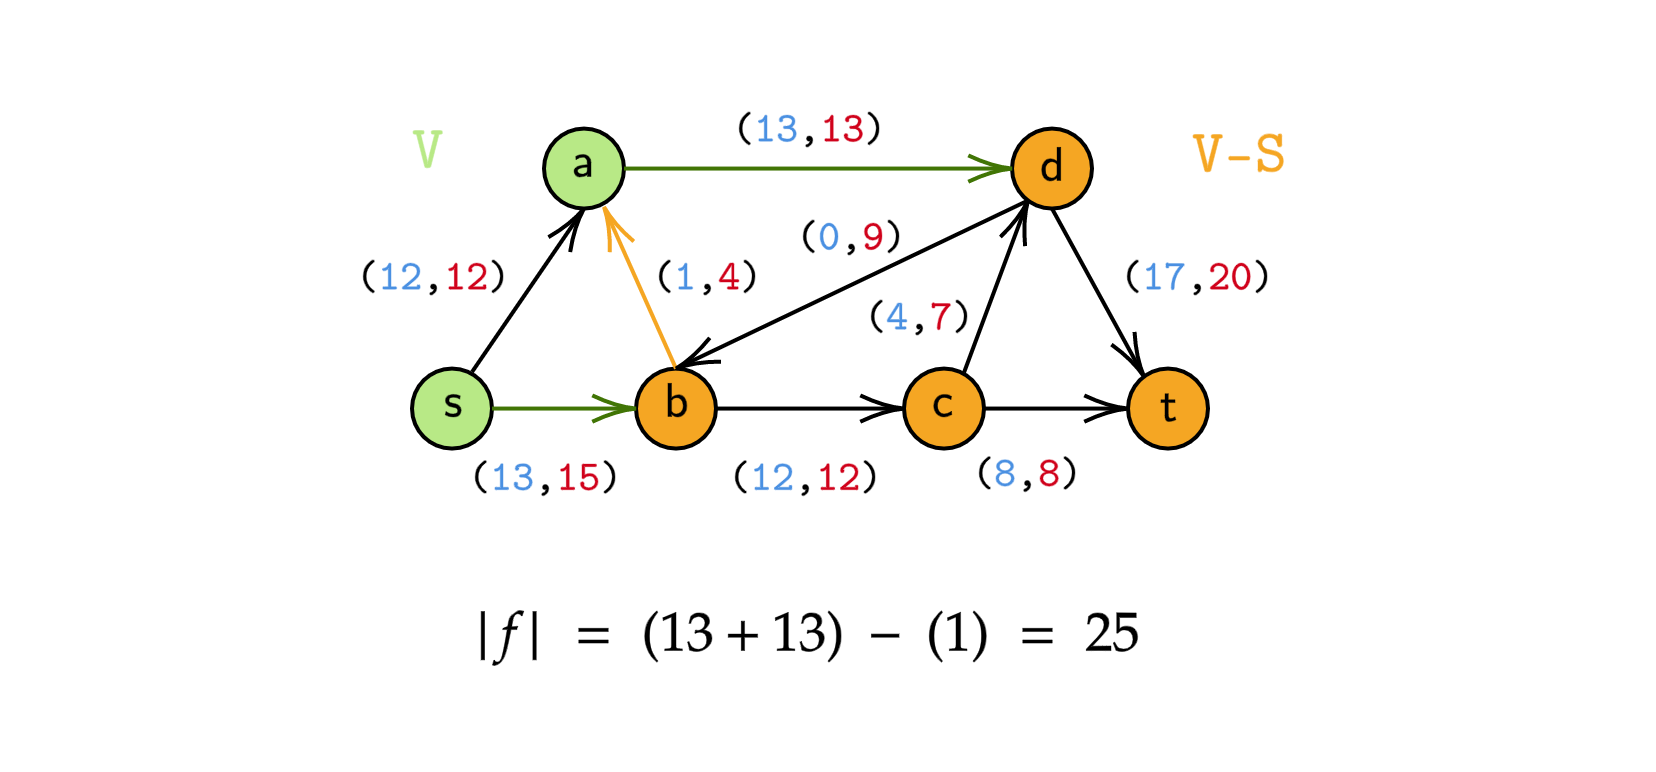
\includegraphics[width=0.8\linewidth]{figures/wk-7/fig-1.jpeg}
    \end{center}

	\begin{center}
    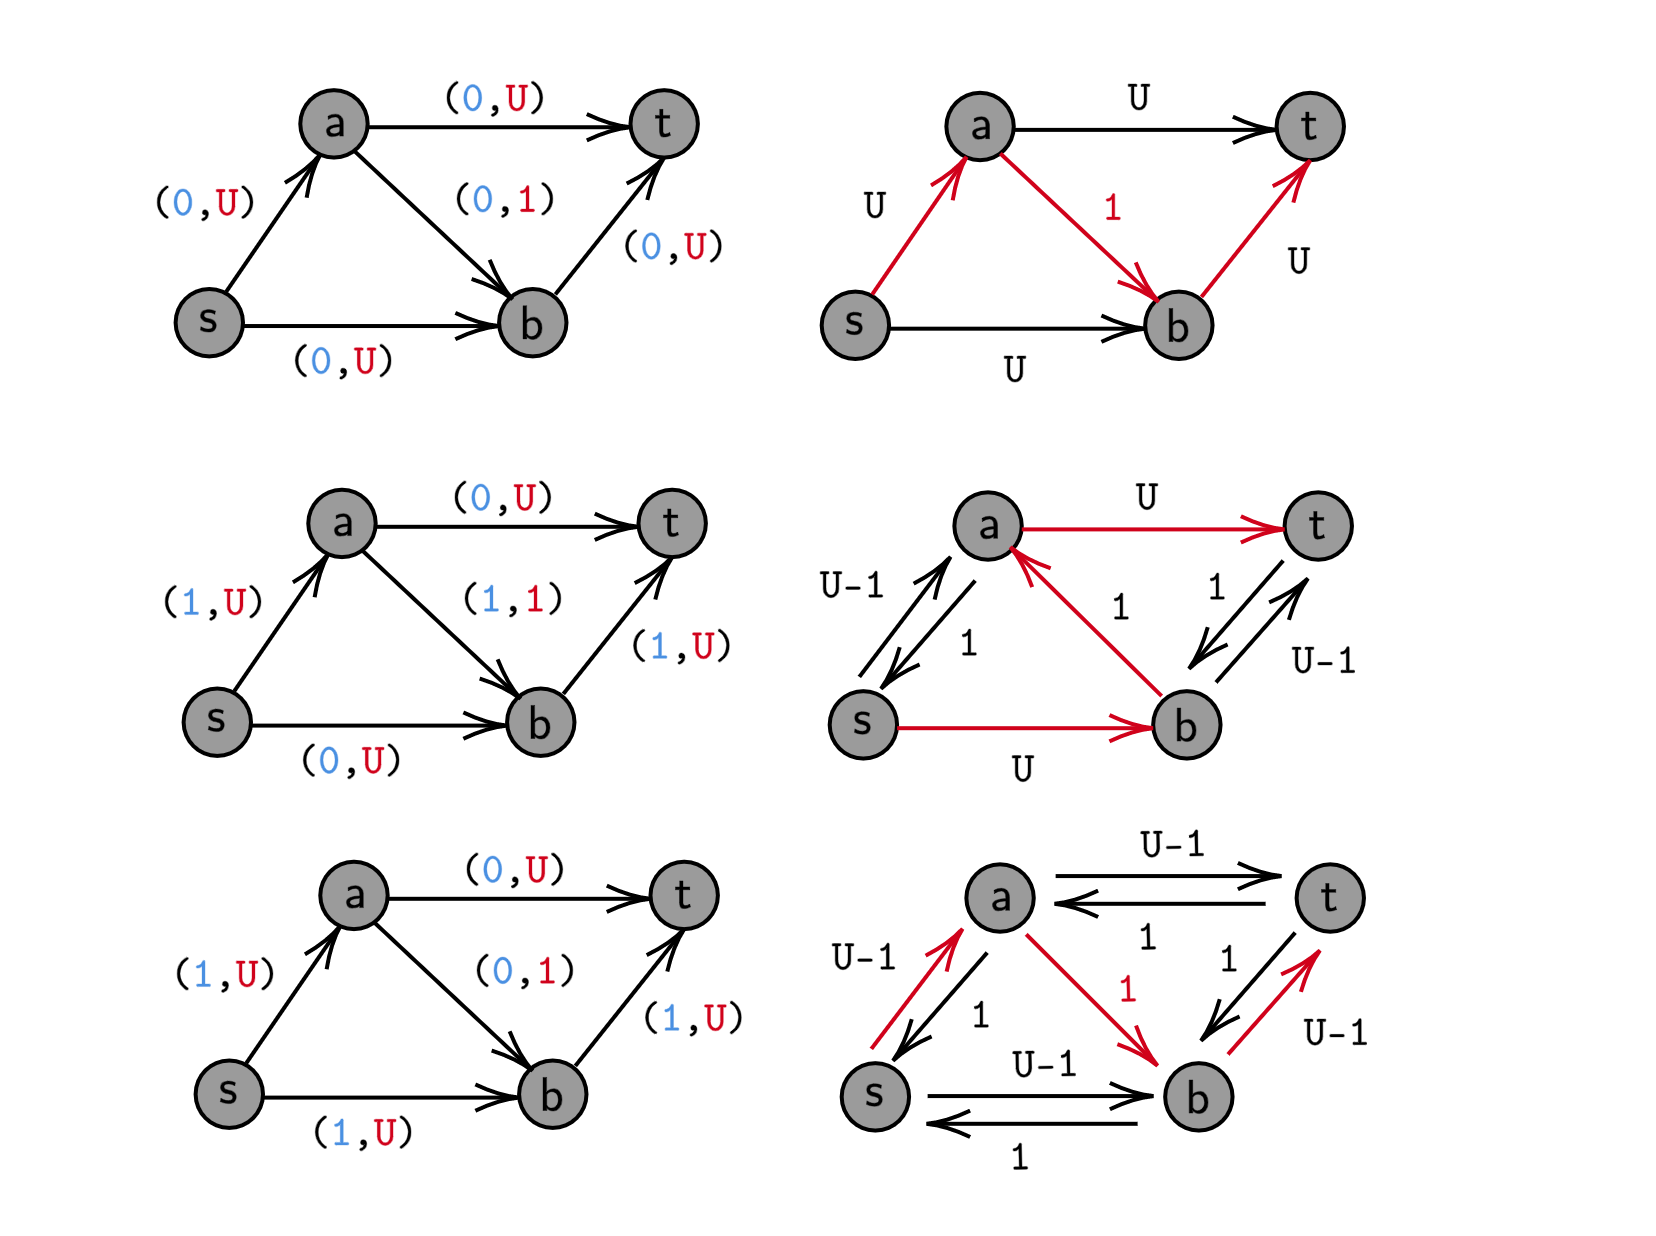
\includegraphics[width=\linewidth]{figures/wk-7/fig-2.jpeg}
    \end{center}

    \begin{rmk}
    	What about $\mathbf{F} = (-y, 0)$, as opposed to $\mathbf{F} = \frac{1}{2}(-y, x)$?
    	\[\begin{aligned}
		&\mathbf{\nabla} \times \mathbf{F}=\left(Q_x-P_y\right) \mathbf{k}=\mathbf{k} \\
		&\Rightarrow \oint_{\left(\partial D^{+}\right)} \mathbf{F} \cdot d \mathbf{s}=\iint_D 1 d x d y
		\end{aligned}\]
		How can we justify without Green's Theorem that,
		\[\oint_c-y d x=\frac{1}{2} \oint_c-y d x+x d y\]
		We have,
		\[\begin{aligned}
		&\mathbf{F_1}:=\frac{1}{2}(-y, x) \\
		&\mathbf{F_2}:=(-y, 0)
		\end{aligned}\]
		and we want to show that,
		\[\oint_c \mathbf{F}_1 \mathbf{d s}=\oint_c \mathbf{F}_2 \mathbf{d s}\]
		which can be accomplished by proving that,
		\[\mathbf{F}_2 - \mathbf{F}_1 = \underbrace{\mathbf{\nabla{V}}}_{=0}\]
    \end{rmk}

 	\begin{center}
    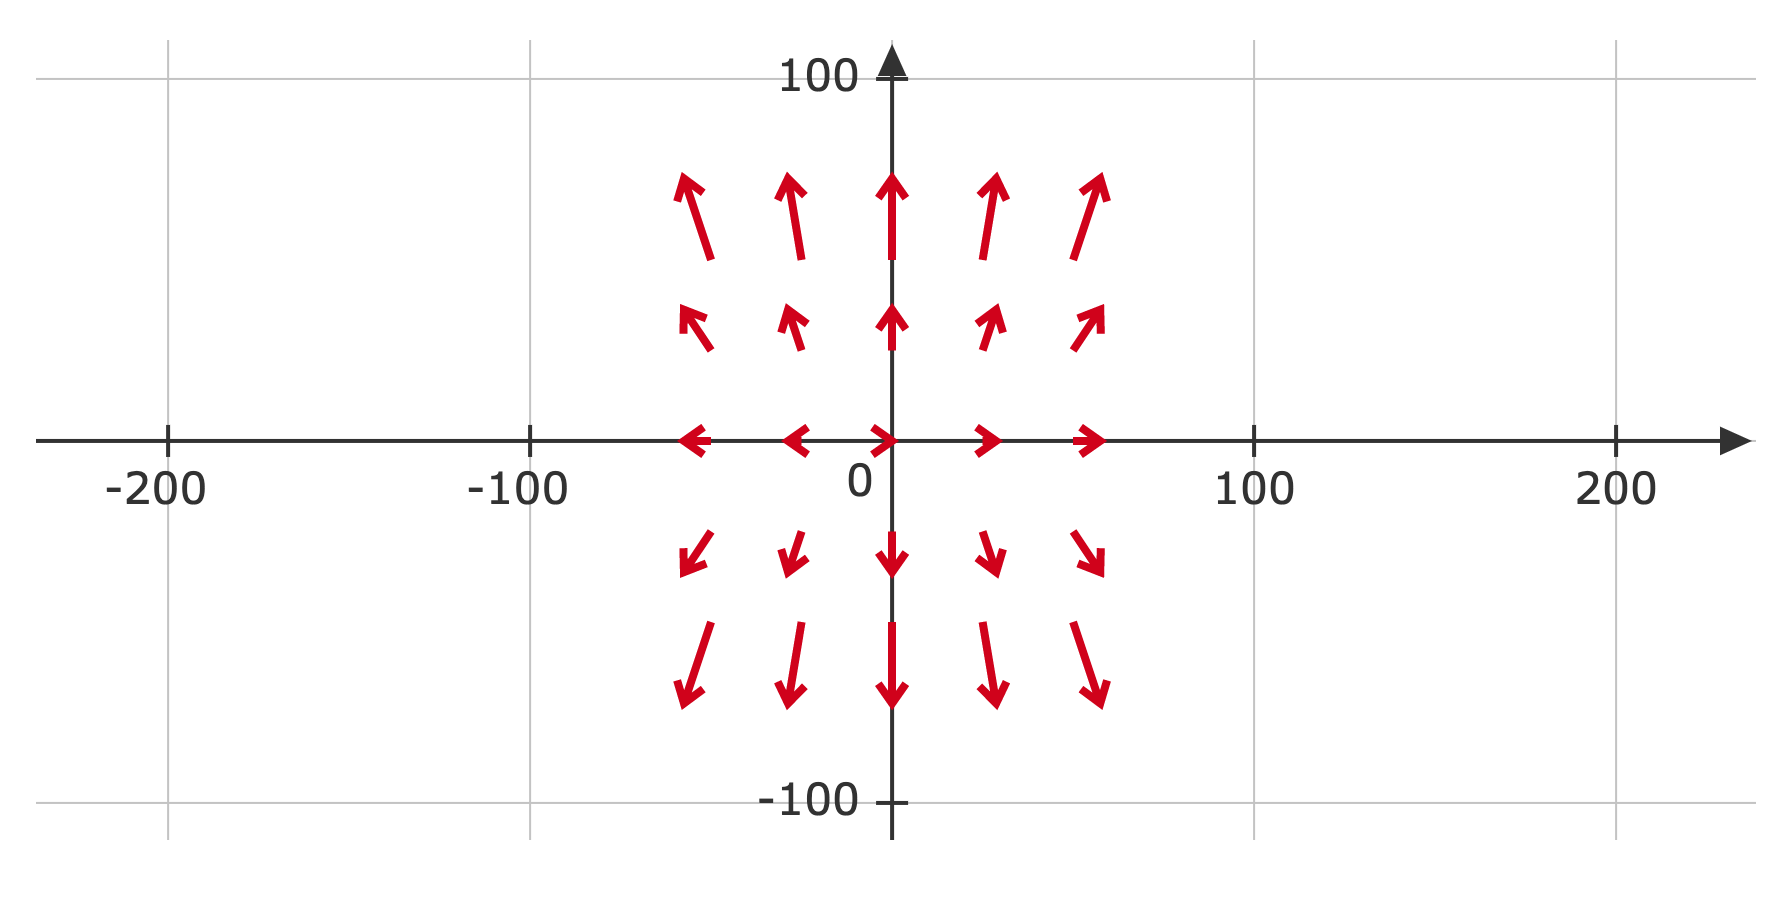
\includegraphics[width=\linewidth]{figures/wk-7/fig-3.jpeg}
    \end{center}